\chapter{Grundlagen neuronaler Netze}
\label{kap:NN}

In diesem Kapitel werden Künstliche Neuronale Netze\cite{dayhoff1990neural}, kurz KNN, als Forschungsgegenstand der Informatik eingeführt und deren mathematische Grundlagen präzisiert. 
Sie stellen informationsverarbeitende Systeme nach dem Vorbild von tierischen beziehungsweise menschlichen Gehirnen dar und bestehen aus Neuronen in gewissen Zuständen und Schichten, die über gewichtete Verbindungen miteinander gekoppelt sind. Jene Gewichte sind als freie Parameter des neuronalen Netzes zu verstehen und können während eines Trainingsprozesses so angepasst werden, um eine entsprechende Aufgabe zu lösen.  
Gelingt dies, so können neuronale Netze genutzt werden, um bestimmte Muster in Daten, typischerweise in Bildern, Audio oder Stromdaten, zu erkennen\cite{pandya1995pattern, pao1989adaptive, urbaniak2021quality}.
Sie eignen sich daher für viele typische Aufgaben des maschinellen Lernens, beispielsweise für die Klassifikation digitalisierter Objekte.

Im ersten Abschnitt wird das Perzeptron\cite{rosenblatt1958perceptron} als Grundeinheit eines neuronalen Netzes eingeführt. 
Im folgenden Abschnitt wird das Konzept der Multi-Layer-Perzeptronen\cite{werbos1988generalization} durch die Kopplung mehrerer Perzeptronen mit bestimmten Übertragungs- und Aktivierungsfunktion in einem Netz erläutert. Diese Repräsentierung eines KNN wird im weiteren Verlauf dieser Arbeit genutzt. Weiter wird das Training neuronaler Netze hinsichtlich der Klassifikationsaufgabe im Abschnitt \ref{abs:task_training} erläutert und schließlich eine kurze Zusammenfassung im letzten Abschnitt \ref{abs:NN_conc} gegeben.

\section{Das Perzeptron}
\label{perzeptron_abs}
Zunächst wird das \textit{Perzeptron} ähnlich wie in Minsky\cite{minsky2017perceptrons} als fundamentaler Baustein eines neuronalen Netzes eingeführt. Das Perzeptron wird oft als Basis moderner KNN angeführt und kann mithilfe des Perzeptron-Lernalgorithmus \ref{alg:pla} trainiert werden, um das Problem der linearen Trennbarkeit von Punktmengen zu lösen.
\begin{defi}[Perzeptron]
    \label{def_neuron}
    Für eine gegebene Funktion $\phi: \RR \rightarrow \RR$, einen Vektor $w \in \Rnv$ und ein Skalar $\theta \in \RR$ wird die Funktion 
    \[ \
    \Phi: \RR^n \rightarrow \RR, \; \; \; x \mapsto \phi(w^T x -\theta)=:y,
    \]
    \textit{Perzeptron} genannt. Mit $x \in \Rnv$ wird die vektorwertige Eingabe und mit $y \in \RR$ die skalare Ausgabe, auch Aktivierung, des Perzeptrons bezeichnet. Dabei ist $w^Tx=\sum_{i=1}^n w_i x_i$ das Standardskalarprodukt im euklidischen Vektorraum $\Rnv$. Die Komponenten von $w$ werden Gewichte und der Skalar $\theta$ Schwellwert oder auch Bias genannt.
\end{defi}
Die Funktionsweise eines Perzeptrons ist in Abbildung \ref{funktionsweise_neuron} dargestellt. In dieser Arbeit wird das Perzeptron oft einfach Neuron genannt. Die Begriffe sind austauschbar und meinen dasselbe.
\begin{figure}[h]
    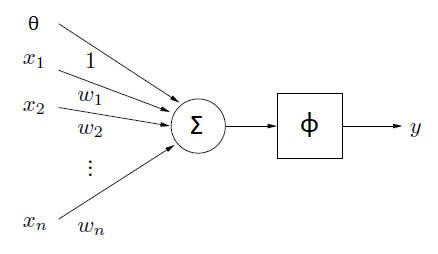
\includegraphics[width=0.8\textwidth]{pics/chapter_neuralnetworks/perzeptron.png}
    \centering
    \caption{Arbeitsweise eines Perzeptrons mit entsprechender Notation aus Definition \ref{def_neuron}.}
    \label{funktionsweise_neuron}
\end{figure}
Bei der Wahl der Funktion $\phi$ gibt es mehrere Möglichkeiten. Wird wie in Minsky\cite{minsky2017perceptrons} die Heavyside-Funktion
\begin{equation*}
    \phi: \RR \rightarrow \RR, \; \; \;
    \phi(x)=\begin{cases}
       1 , \; x \geq 0 \\
       0 , \; \text{sonst}
    \end{cases}
\end{equation*} 
genutzt, kann das Perzeptron als binärer Klassifikator wie in Abschnitt \ref{abs:trenn} interpretiert werden. Dabei dient $w^T x-\theta=0$ als trennende Hyperebene. Ist $w^Tx-\theta<0$, so ist $\psi(x)=0$ und $x$ wird der Klasse $K_{0}$ zugeordnet. Gilt jedoch $w^T x-\theta \geq 0$ und damit $\psi(x)=1$, so ist der Vektor $x$ der Klasse $K_1$ zugehörig. 

Für ein Klassifikationsproblem, bei dem die Klassen nicht linear trennbar sind, scheitern diese einfachen Perzeptronen. Hier wird oft das zweidimensionale XOR-Problem angeführt. Um solche Aufgaben zu lösen, ist es notwendig, mehrere Perzeptronen geschickt zu verknüpfen, um komplexe Entscheidungsgrenzen zu erhalten.

\section{Multi-Layer-Perzeptron}
\label{MLP_abs}
In dieser Arbeit wird ein Künstliches Neuronales Netz als eine Menge von Perzeptronen, die in gewissen Schichten partitioniert und miteinander verbunden sind, notiert. Diese sogenannten \textit{Multi-Layer-Perzeptronen}, kurz MLP,  gelten als erste tiefe neuronale Netze und sind seit den späten 1980er-Jahren Gegenstand der Forschung\cite{bourlard1990links,bounds1988multilayer,MLPbook}. Zunächst sind einige Definition notwendig, vgl. \cite{gruening}, um eine lesbare Notation des MLP zu geben.

\begin{defi}[Übertragungsfunktion]
    \label{def_net}
    Für eine gegebene Matrix $W \in \RR^{n \times m}$ und einen Vektor $b \in \RR^m$ ist 
    \[ 
    \Psi^{W,b}: \RR^n \rightarrow \RR^m, \; \; \; x \mapsto W^T x +b
    \]
    als Übertragungsfunktion definiert. Der Vektor $y=\Psi^{W,b}(x) \in \RR^m $ wird als Netzeingabe bezeichnet.
\end{defi}
Hierbei ist $W$ eine Gewichtsmatrix und $b$ ein Biasvektor, welche als freie Parameter fungieren und die Netzeingabe eines Eingabevektors $x \in \RR^n$ auf lineare Art und Weise beeinflussen. Um auch nichtlineare Zusammenhänge darzustellen, werden Aktivierungsfunktionen benutzt.

\begin{defi}[Aktivierungsfunktion]
    \label{def_act_f}
    Eine stetige, monoton steigende und nicht notwendigerweise lineare Funktion $\psi: \RR \rightarrow \RR$ wird als Aktivierungsfunktion bezeichnet.
\end{defi}
Es sei erwähnt, dass auch nicht monotone Aktivierungsfunktionen genutzt werden können, beispielsweise radiale Basisfunktionen\cite{radialbasis}, welche jedoch in dieser Arbeit nicht weiter von Interesse sind.
Typische Aktivierungsfunktionen, welche heutzutage verwendet werden, sind die:
\begin{align*}
    \text{Identität}: \; \;\psi(x)&=x, \\
    \text{Logistische Funktion}: \; \;\psi(x)&=\frac{1}{1+\mathrm{e}^{-x}}, \\
    \text{Tangens Hyperbolicus}: \; \;\psi(x)&=\tanh(x), \\
    \text{ReLU (rectified linear unit)}: \; \;\psi(x)&=\max\{0,x\}.
\end{align*}

\begin{bem}
    Ist $\psi$ eine Aktivierungsfunktion, so wird für $x \in \RR^n$ mit 
    \[\psi(x):=\left(\psi(x_1), \ldots, \psi(x_n)\right)^T \in \RR^n
    \]
    der Vektor bezeichnet, welcher sich durch die elementweise Auswertung der Aktivierungsfunktion $\psi$ an den Stellen $x_1, \ldots, x_n$ ergibt. 
\end{bem}

%Bei Klassifikationsproblemen wird oft die \textit{Softmax}-Funktion\cite{denker1990transforming} genutzt, welche die gesamte Eingabe berücksichtigt. Im Abschnitt \ref{task_training} wird erläutert, warum sich in diesem Fall die Softmax-Funktion eignet.

%\begin{defi}[Softmax-Funktion]
    %Für $x \in \RR^n$ wird die Funktion $\psi: \RR^n \rightarrow (0,1]^n$ mit 
    %\[
        %\psi(x):=\left(\frac{\mathrm{e}^{x_1}}{\sum_{i=1}^n \mathrm{e}^{x_i}}, \ldots,\frac{\mathrm{e}^{x_n}}{\sum_{i=1}^n \mathrm{e}^{x_i}} \right)^T
    %\]
    %als Softmax-Funktion definiert. Die Einträge des Vektors $\psi(x)$ summieren sich zu Eins.  
%\end{defi}

Für den späteren Trainingsprozess ist es nützlich, die Ableitung der verwendeten Aktivierungsfunktion, sofern sie existiert, zur Verfügung zu haben. Zudem ist es möglich, für bestimmte Aktivierungsfunktionen die Ableitung nur mithilfe der verwendeten Funktion zu berechnen.

\begin{lem}
    \begin{itemize}
        \item[(i)] Für die ReLU $\psi(x)=\max\{0,x\}$ gilt
         \[\psi'(x)=\begin{cases}
            0 &, x <0 \\
            1 &, x >0
        \end{cases}. 
        \]
        An der Stelle 0 ist die Ableitung nicht definiert und wird oft mit $\psi'(0)=\frac{1}{2}$ festgelegt.
        \item[(ii)] Für die logistische Funktion $\psi(x)=\frac{1}{1+\mathrm{e}^{-x}}$ gilt
        \[ 
            \psi'(x)=\psi(x)(1-\psi(x)) 
        \]
        für alle $x \in \RR$.
        \item[(iii)] Für den Tangens Hyperbolicus $\psi(x)=\tanh(x)$ gilt
        \[ 
            \psi'(x)=1-\psi^2(x) 
        \]
        für alle $x \in \RR$.
    \end{itemize}
\end{lem}
\begin{proof}
    Einfaches Differenzieren liefert für $(i)$ und $(ii)$ die Resultate. Bei $(iii)$ wird die Darstellung $\tanh(x)=\frac{2}{\mathrm{e}^{2x}+1}$ genutzt und das Differenzieren mittels Quotientenregel führt zur Aussage.
\end{proof}

Ähnlich der Definition des Perzeptrons \ref{def_neuron} wird nun eine Schicht als Verknüpfung von Übertragungsfunktion und Aktivierungsfunktion definiert.

\begin{defi}[Neuronenschicht]
    \label{def:NNlayer}
    Ist $\Psi^{W,b}$ eine Übertragungsfunktion mit den Parametern $W \in \RR^{n \times m}$ und $b \in \RR^m$ sowie $\psi$ eine Aktivierungsfunktion, so wird das Paar $(\Psi^{W,b}, \psi)$ als Neuronenschicht $\mathcal{S}$ bezeichnet. Für eine Eingabe $x \in \RR^n$ ist die Ausgabe $y \in \RR^m$ der Schicht $\mathcal{S}$ durch
    \[y=\psi \circ \Psi^{W,b}(x)= \psi\left(\Psi^{W,b}(x)\right)
        \] 
        gegeben. Die Komponenten $y_i$ werden für $1 \leq i \leq m$ Aktivierungen der Neuronen in der Schicht $\mathcal{S}$ genannt und gleichen jeweils der Ausgabe eines einfachen Perzeptrons wie in Definition \ref{def_neuron}. Eine Schicht besteht also aus $m$ Neuronen $\Phi_i$ mit der Beziehung $y_i=\Phi_i(x)=\phi(W_{i,:}^T x+b_i)$ für $1 \leq i \leq m$.
\end{defi}
Im Hinblick auf MLPs werden nun mehrere Schichten so verbunden, dass die Ausgabe einer Schicht $\mathcal{S}_k$ als Eingabe einer darüberliegenden Schicht $\mathcal{S}_{k+1}$ für ein $k \in \mathbb{N}$ dient. Die Anzahl der Neuronen kann dabei von Schicht zu Schicht variieren. Dementsprechend werden die Dimensionen der beteiligten Gewichtsmatrizen $W^{(k)}$ und Biasvektoren $b^{(k)}$ passend gewählt. 
Um die Notation übersichtlich zu halten, bezeichne $\Psi^{W^{(k)},b^{(k)},\psi_{k}}$ die Schicht $\mathcal{S}_k$ mit $\Psi^{W^{(k)},b^{(k)},\psi_{k}}(x):= \psi_{k} \left(\Psi^{W^{(k)},b^{(k)}}(x)\right)$.

\begin{defi}[Multi-Layer-Perzeptron, vgl. \cite{gruening}]
    \label{def:MLP}
    Für eine gegebene Anzahl $1<l \in \mathbb{N}$ von Schichten $\Psi^{W^{(1)},b^{(1)},\psi_{1}}, \ldots, \Psi^{W^{(l)},b^{(l)},\psi_{l}}$ bezeichne $s_l \in \mathbb{N}$ die Anzahl der Neuronen in Schicht $l$. Für eine Eingabe $x \in \RR^{s_0}$ lässt sich die Ausgabe $y \in \RR^{s_l}$ eines Multi-Layer-Perzeptron  $\Lambda_l: \RR^{s_0} \rightarrow \RR^{s_l}, \; x \mapsto y$ mit $l$ Schichten durch
    \[
        y=\Psi^{W^{(l)},b^{(l)},\psi_{l}} \circ \ldots \circ \Psi^{W^{(1)},b^{(1)},\psi_{1}}(x)
    \]
    berechnen. Dabei gelten für die Gewichtsmatrizen die Dimensionsbedingungen
    \[{}_1W^{(1)}=s_0, \; \; {}_2W^{(l)}=s_l, \; \; \forall i \in [l-1]: \; {}_2W^{(i)}={}_1W^{(i+1)}.
        \] 
    Die Eingabeschicht $\mathcal{S}_0$ besitzt keine Parameter $W$ und $b$ und besteht nur aus dem Eingabevektor $x \in \RR^{s_0}$. Die letzte Schicht $\Psi^{W^{(l)},b^{(l)},\psi_{l}}$ wird als Ausgabeschicht bezeichnet. Weiter werden die Schichten $\mathcal{S}_1, \ldots, \mathcal{S}_{l-1}$ als verdeckte Schichten definiert. Das MLP wird auch Feed-Forward-Netz (FFN)  genannt und die Funktionsauswertung $\Lambda_l(x)$ für eine Eingabe $x$ wird mit Vorwärtsrechnung, engl. \textit{forward propagation}, bezeichnet.
\end{defi}

\begin{algorithm}
    \caption{Vorwärtsrechnung}\label{alg:ff}
    \begin{algorithmic}
    \Require $ \text{MLP} \; \Lambda_l, \text{Eingabe} \; x_0 \in \RR^n$
    \Ensure $y = \Lambda_l(x) \in \RR^m$
    \State $x=x_0$
    \For{$i=1, \ldots l}$
    \State $u=W^{(i) \,T}x+b^{(i)}$
    \State $x=\psi_i(u)$
    \EndFor
    \State $y=x$
    \end{algorithmic}
\end{algorithm}
    


Das MLP-Modell wird im weiteren Verlauf dieser Arbeit repräsentativ als Künstliches Neuronales Netz bezeichnet. Die Begriffe KNN, MLP und FFN sind austauschbar und meinen dasselbe Modell. Die Funktionsauswertung eines FNN wird im Algorithmus Vorwärtsrechnung \ref{alg:ff} festgehalten. Das zuvor angesprochene XOR-Problem kann nun beispielsweise mithilfe eines FNN bestehend aus zwei Schichten gelöst werden\cite{Goodfellow-et-al-2016}.
Es lassen sich zwischen Modell- und Hyperparameter von KNN unterscheiden.

\begin{defi}[Hyper- und Modellparameter]
    Sei für $l \in \mathbb{N}$ ein FNN $\Lambda_l$ gegeben. Dann werden die Eingabe- und Ausgabedimension $s_0, s_l$, die Anzahl $l$ der (verdeckten) Schichten sowie die verwendeten Aktivierungsfunktion $\psi_l$ Hyperparameter des neuronalen Netzes genannt.
    Die Gewichtsmatrizen und Biasvektoren mit den entsprechend passenden Abmessungen stellen die Modellparameter $\mathcal{W}:=\{(W^{(i)},b^{(i)}): \; i=1, \ldots, l\}$ des neuronales Netzes dar. 
\end{defi}
Die Hyperparameter werden oft anwendungsspezifisch für das jeweilige Problem gewählt, während die Modellparameter dynamisch in einem Trainingsprozes angepasst werden, sodass die gegebene Aufgabe zufriedenstellend gelöst wird. Wie optimale Modellparameter in einem Trainingsprozes gefunden werden können, wird im folgenden Abschnitt \ref{abs:task_training} erläutert.

\section{Optimale Parameterwahl bei neuronalen Netzen}
\label{abs:task_training}
%Künstliche Neuronale Netze gehören zu den typischen Vertretern von maschinellen Lernalgorithmen, welche hinsichtlich einer bestimmten Aufgabe, engl. \textit{task T}, und einem Leistungsmaß, engl. \textit{perfomance P} an der Erfahrung, engl. \textit{experience E} lernen\cite{Goodfellow-et-al-2016}. Dabei ist mit Lernen gemeint, dass das Computerprogramm bezüglich der Aufgabe $T$ sein Leistungsmaß $P$ mit wachsener Erfahrung $E$ schrittweise steigert. Wie in Kapitel \ref{kap:fund} erläutert, gibt es viele verschiedene Aufgaben, wie die Regression, Klassifikation oder Clusterung bestimmter Objekte. 

In diesem Abschnitt steht das Klassifikationsproblem für digitalisierte Objekte im Mittelpunkt. Dazu werden FNN als Modelle $\tilde{f}$ zur Approximation von Klassifikationsfunktionen $f: \mathcal{M} \rightarrow \mathcal{C}$, vgl. Abschnitt \ref{abs:classtask}, eingesetzt. Die Anzahl der Neuronen in der Ausgabeschicht entspricht der Anzahl der verschiedenen Klassen in $\mathcal{C}$, also $s_l=s$. Zur Vereinfachung der Notation sei mit $C:=\{1, \ldots, s\}$ die Menge der Klassen bezeichnet. Wird für eine Eingabe $x$ die Vorwärtsrechnung $\Lambda(x)$ vorgenommen, so bezeichne $\tilde{f}(x)$ die approximierte Klassifikationsfunktion, welche als
\begin{equation*}
    \tilde{f}(x):= \underset{k}{\mathrm{argmax}} \; \left(\Lambda(x)\right)_k
\end{equation*}
definiert ist. Dabei sei bemerkt, dass der Index $l$, welcher die Anzahl der Schichten von $\Lambda$ kodiert, für die folgenden Betrachtungen entfällt.   
Weiter stehe eine Trainingsmenge 
\begin{equation*}
    \mathcal{T}= \{(x_i, c) \in \mathcal{M} \times \mathcal{C}\; : \; 1 \leq i \leq m\}  
\end{equation*}
zur Verfügung. Für ein Trainingspaar $\left(x,c\right) \in \mathcal{T}$ bezeichne $t(x,c) \in \RR^s$ den Zielvektor der Klasse $c$ mit sogenannter (1 aus s)-Kodierung. Die Komponenten des Zielvektors sind
\begin{equation*}
    t_k(x,c):= \begin{cases}
        1 &, \text{wenn} \; k=c \\
        0 &, \text{sonst}
    \end{cases}, \; \; \forall k \in [s].
\end{equation*} 
Sind die Hyperparameter des FFN festgelegt, müssen die Modellparameter $\mathcal{W}$ optimal gewählt werden. In diesem Sinne bedeutet optimal, dass das Minimierungproblem 
\begin{equation}
    \label{eq:Emin}
    \mathcal{E}(\mathcal{T}, \mathcal{W}) \rightarrow \min
\end{equation} 
im Raum der Parameter $\mathcal{W}$ gelöst werden soll. Dabei sei bemerkt, dass dies unabhängig von den Hyperparametern geschieht. Im Folgenden wird der Backpropagationsalgorithmus als ein Lösungsansatz für Aufgabe (\ref{eq:Emin}) vorgestellt.  
%Um die Approximationsgüte, also die \textit{perfomance P}, bezüglich des Klassifikationsproblems messbar zu machen, werden Fehlerfunktionen eingeführt. 
%Mit Trainingsdaten als \textit{experience E} und dem Gradientenverfahren\cite{nocedal1999numerical} sollen optimale Parameter $\mathcal{W}$ gefunden werden, sodass die gewählte Fehlerfunktion minimiert wird. Im folgenden steht ein MLP $\Lambda(\, \cdot \, ; \mathcal{W}): D \rightarrow [0,1]^m$  mit der Softmax-Funktion als Aktivierungsfunktion im Mittlepunkt, welches als parametrisiertes Modell $f_{Modell}$ wie in \ref{eq:f_modell} genutzt wird.
%Die Trainingsdaten werden in Trainingsmengen und Testmengen aufgeteilt.

%\begin{defi}[Trainingsmenge, Testmenge]
    %Sei $p_{daten}$ eine Datenverteilung auf der Ergebnismenge $\Omega=D \times \mathcal{C}$. Dann heißen für $n_{train}, n_{test} \in \mathbb{N}$ die Mengen
    %\begin{align*}
     %   \mathcal{T} &:= \left\{ (x^{(i)},c^{(i)}) \; | \; i \in [n_{train}] \right\} \subset \Omega \\
     %   \mathcal{T}' &:= \left\{ (x^{(i)},c^{(i)}) \; | \; i \in [n_{test}] \right\} \subset \Omega
    %\end{align*}
    %Traingsmenge $\mathcal{T}$ und Testmenge $\mathcal{T}'$, jeweils bestehend aus Datenpaaren, welche unabhängig durch $p_{Daten}$ generiert wurde. Oft werden die Mengen disjunkt gewählt. Die Menge $\mathcal{T}$ wird zum Trainieren und die Menge $\mathcal{T}'$ zur Validierung des Modells $P_{Modell}$ bezüglich $P_{Daten}$ wie in \ref{eq:Pdaten} genutzt.
%\end{defi}

%Die Approximationsgüte des Modells $f_{Modell}$ wird als Likelihood gegeben einer Trainingsmenge $\mathcal{T}$ gemessen und lässt sich als 

%\begin{equation}
 %   \label{eq:likelihood}
  %  L(\mathcal{T},\mathcal{W}):=\prod_{(x,c) \in \mathcal{T}} p_{Modell}(c \; | \; x; \mathcal{W})
%\end{equation}
%wie in Bishop\cite{bishop2006pattern} berechnen.
%Für eine Trainingsmenge $\mathcal{T}$ soll das Produkt über alle Wahrscheinlichkeiten der korrekten Klassenzugehörigkeiten $c$ gegeben der Eingaben $x$ maximiert werden. Dieser Ansatz wird \textit{Maximum Likelihood-Methode}\cite{ruschendorf2014mathematische} genannt und eine Parameterwahl ist durch eine Lösung des Optimierungsproblems 
%\begin{equation}
    %\label{eq:opt_likelihood}
    % \prod_{(x,c) \in \mathcal{T}} p_{Modell}(c \; | \; x; \mathcal{W}) \rightarrow \max
%\end{equation}

%Mit dieser Bezeichnung lässt sich das Optimierungsproblem \ref{eq:opt_likelihood} als Minimierungproblem mithilfe der \textit{negative log likelihood} schreiben.
%\begin{defi}[negative log likelihood]
    %Seien die Mengen $D$ und  $\mathcal{C}=\{c_1, \ldots, c_m\}$ mit einer dazugehörigen Trainingsmenge $\mathcal{T}$ sowie entsprechende Zielvektoren gegeben. Weiter seien die a posterior Wahrscheinlichkeiten $p_{Modell}(c \; | \; x; \mathcal{W})$ wie in Gleichung \ref{eq:Pmodell} gegeben. Die negative log likelihood ist als Funktion 
    %\begin{equation}
    %    \label{eq:NLL}
     %   L_{NNL}(\mathcal{T},\mathcal{W}):= -\sum_{(x,c) \in \mathcal{T}}  \sum_{i=1}^m t_i(x,c) \log \left(p_{Modell}(c_i \; | \; x; \mathcal{W}) \right) 
    %\end{equation}
   % definiert.
%\end{defi}

%Das Minimieren der negative log likelihood ist äquivalent zur Maximierung der Likelihood aus \ref{eq:likelihood}, denn es gilt 
%\begin{equation*}
    %\log \left(\prod_{(x,c) \in \mathcal{T}} p_{Modell}(c \; | \; x; \mathcal{W})\right)= \sum_{(x,c) \in \mathcal{T}} \log \left(p_{Modell}(c \; | \; x; \mathcal{W}) \right)
%\end{equation*}
%und der natürliche Logarithmus ist monoton steigend. Wird zusätzlich angenommen, dass die a posterior Verteilung  $p_{Daten}(c \; | \; x)$ einer Normalverteilung mit konstanter Varianz entspricht, so ist das Maximieren von \ref{eq:likelihood} äquivalent zur Minimierung der mittleren quadratischen Abweichung


 \section*{Backpropagationsalgorithmus}
Bei FFN wird Backpropagation, etabliert von Rumelhart et. al. \cite{MLPbook}, als Lernalgorithmus genutzt, um eine gewählte Fehlerfunktion $\mathcal{E}$ zu minimieren. Dabei wird das Gradientenverfahren, vgl. Algorithmus \ref{alg:gradver}, zur numerischen Minimierung von $\mathcal{E}$ im Raum der Modellparameter $\mathcal{W}$ genutzt. Es sei bemerkt, dass das Finden von globalen Minima durch den Backpropagationsalgorithmus keineswegs garantiert ist.
In dieser Arbeit wird $\mathcal{E}$ immer als stetig differenzierbare Funktion vorausgesetzt, damit das Gradientenverfahren angewendet werden kann. Ebenso sollten alle verwendeten Aktivierungsfunktionen aus Definition \ref{def_act_f} als stückweise stetig differenzierbare Funktion vorausgesetzt werden. 
Die Optimierung der Parameter geschieht iterativ, dargestellt mit dem Index $n$, und besteht aus zwei Schritten. Für festes $n$ wird zuerst eine Abstiegsrichtung 
\begin{equation}
    \label{eq:gradE}
    \Delta_n := \nabla_{\mathcal{W}} \mathcal{E}(\mathcal{T},\mathcal{W})
\end{equation} 
berechnet und dann werden die Parameter 
\begin{equation}
    \label{eq:step}
    \mathcal{W}_{n+1}:=\mathcal{W}_n + \lambda \Delta_n
\end{equation}
aktualisiert. Es werden Gradienten der Fehlerfunktion bezüglich der Gewichtsmatrizen und Biasvektoren ermittelt und anschließend werden jene Parameter mit einer wählbaren Lernrate $\lambda \in \RR$ in (\ref{eq:step}) angepasst. In (\ref{eq:gradE}) wird der Gradient über alle Trainingspaare berechnet. Diese Variante nennt sich \textit{Offline-Version} des Gradientenverfahrens und ist besonders für große Trainingsmengen ineffizient. Die \textit{Online-Version} berechnet den Gradienten lediglich für ein Trainingspaar und passt die Parameter direkt an. Ein Kompromiss aus beiden Verfahren ist das \textit{Mini-Batch-Verfahren} bei dem die Gradienten über kleine Teilmengen $\mathbb{T} \subset \mathcal{T}$ der Trainingsmenge berechnet werden.
Die Abstiegsrichtungen werden mithilfe der mehrdimensionalen Kettenregel  berechnet.
\begin{satz}[Mehrdimensionale Kettenregel]
    \label{s:chainrule}
    Ist $f=f(x_1(y_1, \ldots, y_m), \ldots, x_n(y_1, \ldots, y_m))$ und sind alle beteiligten Funktionen stetig differenzierbar, so ergeben sich die partiellen Ableitungen mittels Kettenregel zu

    \begin{equation*}
        \frac{\partial f}{\partial y_i}=\sum_{j=1}^n \frac{\partial f}{\partial x_j} \frac{\partial x_j}{\partial y_i} .
    \end{equation*}
\end{satz}

\begin{proof}
    Ein Beweis kann in Forster \cite{forster2017analysis} gelesen werden.
\end{proof}
Die effiziente Berechnung der Abstiegsrichtungen gehört zu den schwersten Aufgaben des Maschinellen Lernens, siehe \cite{DBLP:series/lncs/LeCunBOM12}.
Der Online-Backpropagationsalgorithmus, in der Literatur auch als \textit{Stochastic Gradient Descent} bezeichnet, wird im Folgenden zur Optimierung der Modellparameter erläutert. Grundsätzlich lässt sich das Verfahren in zwei Schritte einteilen.

\begin{itemize}
    \item Bei der Vorwärtsrechnung wird dem FFN $\Lambda$ ein Trainingspaar ($x,c) \in \mathcal{T}$ präsentiert und die Aktivierungen der Schichten schrittweise von der Eingabeschicht über die verdeckten Schichten bis zur Ausgabeschicht berechnet. Der Fehler in der Ausgabeschicht wird mithilfe einer Fehlerfunktion $\mathcal{E}$ berechnet.
    \item Bei der Rückwärtsrechnung wird für jedes Neuron ein lokaler Fehler bezüglich $\mathcal{E}$ berechnet, beginnend in der Ausgabeschicht über die verdeckten Schichten bis zur Eingabeschicht. Der Fehler wird über die Ausgabe- zur Eingabeschicht zurück propagiert. Dabei werden die Gewichtungen der Neuronenverbindungen und Schwellwerte abhängig von ihrem Einfluss auf den Fehler dirket bzw. indirekt geändert.
\end{itemize}
%\begin{equation*}
%    \label{eq:MSE_1}
%    L_{MSE}(\mathcal{T},\mathcal{W}):=\frac{1}{2} \sum_{(x,c) \in \mathcal{T}} ||\hat{c}-t(x,c)||_2^2,
%\end{equation*}
%wobei $\hat{c}=f_{Modell}(x)$ und $t(x,c)$ der Zielvektor des Datenpaars $(x,c)$ ist.
%Das Problem \ref{eq:opt_likelihood} wird nun allgmemein mit Fehlerfunktionen definiert.
% \begin{defi}[Fehlerfunktion]
 %   Seien $\mathcal{T}$ eine Trainingsmenge und $\mathcal{W}$ Modellparameter eines KNN. Es soll das Problem
  %  \begin{equation}
   %     \label{eq:error_fun_opt}
    %    E(\mathcal{T},\mathcal{W}) \rightarrow \min
    %\end{equation}
    %gelöst werden. Dabei wird $\mathcal{E}$ Fehlerfunktion gennant.
 %\end{defi}
Als Fehlerfunktion $\mathcal{E}$ wird im weiteren Verlauf die mittlere quadratische Abweichung verwendet.
\begin{defi}
    \label{def:MSE}
    Seien eine Trainingsmenge $\mathcal{T}$ und Modellparameter $\mathcal{W}$ eines FFN $\Lambda$ gegeben. Dann wird die mittlere quadratische Abweichung als
\begin{equation*}
    E(x, \mathcal{W}):=\frac{1}{2} \sum_{(x,c) \in \mathcal{T}} ||y-t||_2^2,
\end{equation*}
definiert, wobei $y=\Lambda(x)$ der Ausgabevektor des FFN und $t=t(x,c)$ der Zielvektor des Datenpaars $(x,c)$ ist.
\end{defi}

Beim Online-Verfahren wird der Fehler 
\begin{equation}
    \label{eq:MSE_single}
    E_x= \frac{1}{2} ||y-t(x,c)||_2^2= \frac{1}{2} \sum_{k=1}^{s_l} (y_k-t_k)^2
\end{equation}
für eine einzige Eingabe $x$ berechnet. Es müssen die Abstiegsrichtungen 
\begin{align*}
    \Delta_{W^{(m)}} &= \frac{\partial E_x}{\partial W^{(m)}} \\
    \Delta_{b^{(m)}} &= \frac{\partial E_x}{\partial b^{(m)}} 
\end{align*}
für $1 \leq m \leq l$ ermittelt werden. Die Ausgabeschicht eines $l$-schichtigen FFN $\Lambda$ besitze $s_l$ Neuronen. Im Folgenden wird die Notation wie in \cite{du_diss} mit
\begin{alignat*}{3}
    &w_{k,j}^l  &&\text{Eintrag der Gewichtsmatrix $W^{(l)}$ der Ausgabeschicht}, \\
    &w_{j,i}^h   &&\text{Eintrag der Gewichtsmatrix $W^{(h)}$ einer verdeckten Schicht}, \\
    &V_j=\sum_{i} w_{j,i}^h x_i +b^h_j \; \; \;  &&\text{Netzeingabe des verdeckten Neurons $j$ mit Bias $b^{(h)}$}, \\
    &z_{j}= \psi \left(V_j\right) &&\text{Aktivierung des Neurons $j$},\\
    &V_k=\sum_{j} w_{k,j}^l z_j +b^l_k&&\text{Netzeingabe des Ausgabeneurons $k$ mit Bias $b^{(l)}$}, \\
    &y_k=\psi(V_k) &&\text{Aktivierung des Ausgabeneurons} \; k,\\
    &e_k=y_k-t_k &&\text{Fehler des $k$-ten Ausgabeneurons} 
\end{alignat*}
genutzt. Zunächst wird nur eine verdeckte Schicht mit $s_j$ Neuronen betrachtet. 
%ie Verallgemeinerung für beliebig viele Schichten ist analog. 
Mit $i$ ist ein Eingabeneuron, $j$ eine verdecktes Neuron und $k$ eine Ausgabeneuron gemeint. Außerdem werden die Gradienten komponentenweise berechnet und daher die Modellparameter komponentenweise aktualisiert. Das mehrmalige Anwenden der Kettenregel \ref{s:chainrule} auf die Fehlerfunktion (\ref{eq:MSE_single}) liefert
\begin{align*}
    \label{eq:delta_w_out}
\Delta w_{k,j}^l &= \frac{\partial E_x}{\partial w_{k,j}^l} \\
                 &= \frac{\partial E_x}{\partial e_{k}}
                            \frac{\partial e_k}{\partial y_k} 
                            \frac{\partial y_k}{\partial V_k}
                            \frac{\partial V_k}{\partial w_{k,j}^l}\\
                 &= e_k \psi'(V_k) z_j \\
                 &= \delta_k z_j           
\end{align*} 
mit 
\begin{equation*}
    \label{eq:delta_out}
    \delta_k:= e_k \psi'(V_k)=\frac{\partial E_x}{\partial V_k}
\end{equation*}
als sogenannte lokale Fehler für $1 \leq k \leq s_l$. Für die Ausgabeschicht lässt sich der lokale Fehler direkt berechnen.
Für die Schwellwerte gilt analog
\begin{equation*}
    \Delta b_k^l =  \frac{\partial E_x}{\partial b_{k}^l} 
                 =  \delta_k.
\end{equation*}
Die lokalen Fehler bzg. $E_x$ für die Parameter der verdeckten Schicht lassen sich indirket mithilfe der lokalen Fehler $\delta_k$ der darüberliegenden Ausgabeschicht berechnen. Es gilt
\begin{align*}
    \Delta w_{j,i}^h &= \frac{\partial E_x}{\partial w_{j,i}^h} \\
                     &= \frac{\partial E_x}{\partial z_{j}}
                            \frac{\partial z_j}{\partial V_j} 
                            \frac{\partial V_j}{\partial w_{j,i}^h} \\
                    &= ,\left( \sum_{k=1}^{s_l} e_k \frac{\partial e_k}{\partial z_j}\right) \psi'(V_j) x_i \\
                    &= \left( \sum_{k=1}^{s_l} e_k \frac{\partial e_k}{\partial y_k} \frac{\partial y_k}{\partial V_k} \frac{\partial V_k}{\partial z_j}\right) \psi'(V_j) x_i \\
                    &= \left( \sum_{k=1}^{s_l} e_k \psi'(V_k) w_{k,j}^l \right) \psi'(V_j) x_i \\
                    &=  \delta_j x_i
\end{align*}
mit $x_i$ als Eingabeneuron und
\begin{equation}
    \label{eq:delta_hidden}
    \delta_j:= \left(\sum_{k=1}^{s_l} \delta_k w_{k,j}^l\right) \psi'(V_j)=\frac{\partial E_x}{\partial V_j}
\end{equation}
als lokale Fehler der verdeckten Neuronen für $1 \leq j \leq s_j$. Hier werden die lokalen Fehler bezüglich $E_x$ von der darüberliegenden Schicht zurück propagiert.
Für die Schwellwerte gilt wieder
\begin{equation*}
    \Delta b_j^h =  \frac{\partial E_x}{\partial b_{j}^h} 
                 =  \delta_j.
\end{equation*}

\subsection*{Backpropagation für mehrere Neuronenschichten}
Die Verallgemeinerung für beliebig viele verdeckte Schichten lässt sich in Abhängigkeit der lokalen Fehler beschreiben. Zur Vereinfachung der Notation beschreibe $L$ die Anzahl der Neuronenschichten eines FFN $\Lambda_L$. Seien mit $w^{(l)}_{j,i}$ und $b^{(l)}_j$ Parameter einer beliebigen Neuronenschicht $l$ bezeichnet. Dann gilt 
\begin{align*}
    \Delta w^{(l)}_{j,i}&= \frac{\partial E_x}{\partial w^{(l)}_{j,i}}= \delta^{(l)}_j z^{(l-1)}_i \\
    \Delta b^{(l)}_{j}&= \frac{\partial E_x}{\partial b^{(l)}_{j}}= \delta^{(l)}_j
\end{align*}
mit 
\begin{equation*}
    \delta^{(l)}_j=
    \begin{cases}
        e_j \psi'(V^{(L)}_j), &\text{wenn $j$ ein Ausgabeneuron ist}, \\
        \left(\sum_{k} \delta^{(l+1)}_k w^{(l+1)}_{k,j}\right) \psi'(V_j^{(l)}), &\text{wenn $j$ ein verdecktes Neuron ist}.
    \end{cases}
\end{equation*}
Dabei ist $z^{(l-1)}_i$ die Aktivierung des Neurons $i$ auf der Schicht $l-1$, $e_j=y_j-t_j$ der Fehler des $j$-ten Ausgabeneurons, $V^{(l)}_j$ die Netzeingabe des $j$-ten Neurons der Schicht $l$, $\delta^{(l+1)}_k= \frac{\partial E_x}{\partial V^{(l+1)}_k}$ der lokale Fehler der Schicht $l+1$ und $w^{(l+1)}_{k,j}$ entsprechende Gewichte. 
Die Online-Backpropagation eines FFN $\Lambda$ wird als komponentenweiser und iterativer Trainingsalgorithmus beschrieben. Daher taucht im Algorithmus \ref{alg:online_backprop} eine Schleife in Abhängigkeit von $n$ auf. Als Abbruchbedingung kann eine maximale Anzahl $N$ von Iterationen vorgegeben werden. Andere Abbruchbedingungen können mit der Norm der Abstiegsrichtungen oder abhängig von der Größe des Traingsfehlers mit einer Fehlertoleranz $\varepsilon >0$ formuliert werden.

\begin{algorithm}[h]
    \caption{Online-Backpropagation für ein FFN $\Lambda_L$}
    \label{alg:online_backprop}
    \begin{algorithmic}
    \Require  Trainingsmenge $\mathcal{T}$, Modellparameter $\mathcal{W}_0$, Fehlerfunktion $E$, Lernrate $\lambda$ 
    \Ensure $\text{optimierte Modellparameter} \; \mathcal{W}$
    \State Initialisiere zufällig alle Gewichte und Schwellwerte des FFN $\Lambda_L$ 
    \State Berechne für die Eingabe $(x,c)$ den Zielvektor $t=t(x,c)$
    \State $n=0$  
    \State $E=\inf$
    \While{$E >\varepsilon$ \textbf{or} $n < N$} \Comment{Abbruchbedingung, siehe Text}
    \For{$(x,c) \in \mathcal{T}$}
        \State Vorwärtsrechnung $y=\Lambda(x)$
        \For{$k=1, \ldots, s_L$}
            \State $\delta_k^{(L)}=(y_k-t_k) \psi'(V^{(L)}_k)$
        \EndFor
        \State Backpropagation
        \For{Schichten $l=L-1, \ldots 1$}
             \For{$j=1, \ldots, s_l$}
                \State $\delta^{(l)}_j= \left(\sum_{k=1}^{s_{l+1}} \delta_k^{(l+1)} w^{(l+1)}_{k,j}\right) \psi'(V^{(l)}_j)$
             \EndFor
        \EndFor 
        \State Berechne Gradienten und aktualisiere Gewichte
        \For{$l=1, \ldots, L$}
        \For{$j=1, \ldots, s_{l}$}
        \For{$i=1, \ldots s_{j-1}$}
        \State $\Delta w_{j,i}^{(l)}= \delta_j^{(l)} z^{(l-1)}_i$
        \State $w^{(l)}_{j,i}= w^{(l)}_{j,i} + \lambda \Delta w_{j,i}^{(l)}$
        \EndFor
        \State $\Delta b^{(l)}_j=\delta^{(l)}_j$
        \State $b^{(l)}_j=b^{(l)}_j + \lambda \Delta b^{(l)}_j$
        \EndFor
        \EndFor
        \State $n=n+1$
    \EndFor
    \State $E=\frac{1}{2} \sum_{(x,c) \in \mathcal{T}} ||y-t||_2^2$
    \EndWhile
    \end{algorithmic}
\end{algorithm}


Bei der Wahl der Lernrate werden heutzutage oft adaptive Verfahren genutzt, welche vorangegangene Gradienten berücksichtigen und die Lernrate so anpassen. Bekannte Verfahren sind \textit{Nesterov accelerated
gradient} \cite{sutskever2013importance}, \textit{AdaGrad} \cite{duchi2011adaptive}, \textit{RMSProp} \cite{tieleman2012lecture} sowie \textit{Adam} \cite{Kingma2015AdamAM}. So sollen Probleme wie des \textit{vanishing gradients} oder des \textit{exploding gradients} vermieden werden, siehe dazu \cite{hanin2018neural}.
Für eine tiefere Analyse des Gradientenverfahrens und dessen Varianten sei auf die jeweilgen Arbeiten beziehungsweise als Zusammenfassung auf Ruder \cite{ruder2016overview,} verwiesen. Darüber hinaus gibt es andere Techniken wie die Regularisierung, um den oben genannten Probleme zu entgehen.
Für die Problemstellung in dieser Arbeit ist es ausreichend, das Online-Verfahren mit konstanter Lernrate zu nutzen. 

\section{Zusammenfassung}
\label{abs:NN_conc}
In diesem Kapitel wurden Feed-Forward-Netze als Modelle eingeführt, um Klassifikationsaufgaben zu lösen. Dabei ist es wichtig die Hyper- und Modellparameter je nach Anwendung und Leistungsmaß optimal zu wählen. Dazu werden Trainingsdaten genutzt, um während eines Lernprozesses eine Fehlerfunktion zu Minimieren. Eine Lösung von (\ref{eq:Emin}) kann wegen der Komplexität allgmemeiner Fehlerfunktion $\mathcal{E}$ bzw. der großen Menge von Parametern $\mathcal{W}$ selten direkt angegeben werden\cite{blum1992training}. Daher wird das Gradientenverfahren als iterativer Ansatz zur numerischen Minimierung der Fehlerfunktion genutzt. Dabei sind partielle Ableitungen der Fehlerfunktion bezüglich der Parameter der Neuronenschichten nötig, welche im Backpropagationsalgorithmus dirket bzw. indirekt mithilfe der mehrdimensionalen Kettenregel berechnet werden können. 

Bei der Analyse von Zeitreihen oder Bildern eignen sich abgewandelte Architekturen wie gefaltete neuronale Netze (CNN), engl. \textit{Convolutional Neural Networks}, welche im folgenden Kapitel \ref{kap:CNN} näher erläutert werden. Diese Art neuronaler Netze wird im weiteren Verlauf dieser Arbeit im Fokus stehen.


    





